\subsection{Task 1: Degree distribution}

\subsubsection{Description}
We conduct 5 experiments on large scale graph data(all with more than 1 million nodes). The details of each dataset is as follows: \\

\begin{center}
\begin{tabular}{| c | c | c |}
    \hline
    name & nodes & edges \\ \hline
    Roadnet-ca & 1,965,206 & 5,533,214 \\ \hline
    Roadnet-PA & 1,088,092 & 3,083,796 \\ \hline
    Roadnet-TX & 1,379,917 & 3,843,320 \\ \hline
    wiki-Talk & 2,394,385 & 5,021,410 \\ \hline
    Youtube & 1,134,890 & 2,987,624 \\ \hline
\end{tabular}
\end{center}


Following(Figure \ref{t1:plot}) are the rank-frequency plots of each dataset, (a)(b) shows the in degree and out degree out Wikitalk. (c) is Roadnet-Ca. (d) is Roadnet-PA. (e) is Roadnet-TX. (f) is Youtube. 

\subsubsection{Plots}

\begin{figure}[!htbf]
\begin{center}
\begin{tabular}{c c c}
     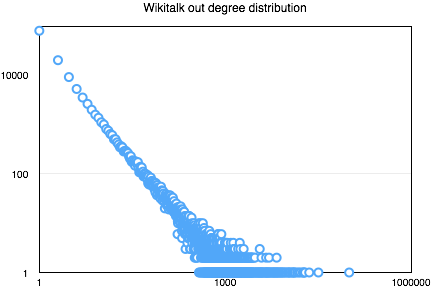
\includegraphics[width=0.3\textwidth]{FIG/t1_wiki_in.png} &
     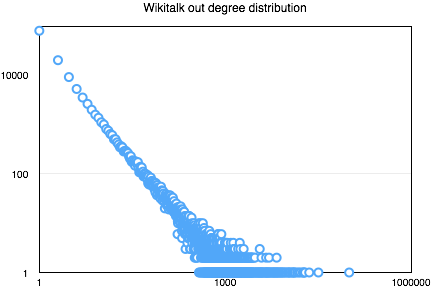
\includegraphics[width=0.3\textwidth]{FIG/t1_wiki_out.png} & 
     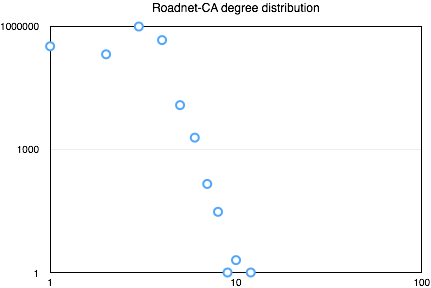
\includegraphics[width=0.3\textwidth]{FIG/t1_ca.png}\\
    (a) & (b) & (c) \\
     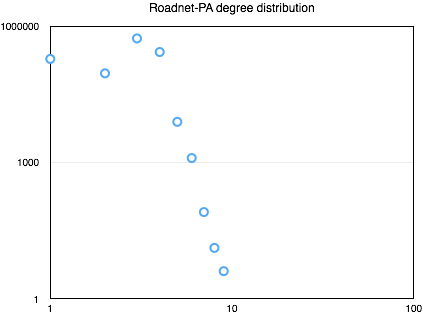
\includegraphics[width=0.3\textwidth]{FIG/t1_pa.png} & 
     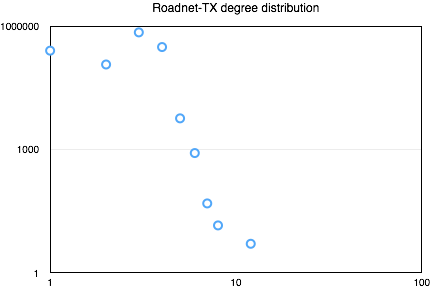
\includegraphics[width=0.3\textwidth]{FIG/t1_tx.png} & 
     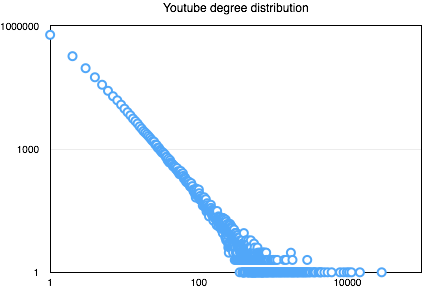
\includegraphics[width=0.3\textwidth]{FIG/t1_youtube.png} \\
     (d) & (e) & (f) \\
\end{tabular}
\caption{In degree distribution (a) and out degree distribution (b) of Wikitalk (c) Roadnet-CA, (d) Roadnet-PA (e) Roadnet-TX (f) Youtube}
\label{t1:plot}
\end{center}
\end{figure}

\subsubsection{Observation}
As we can observe, that most \emph{social network} exhibit perfect power law in degree distribution. It aligned with our intuition. While for the series of Roadnet dataset, we can not observe obvious power law. So maybe we can conclude that not all graphs have power law property in it. Some datasets like roadnet, involves a lot of human design, is less \emph{chaotic} than ordinary graphs.